\chapter{Host Compiled Simulation}

\gls{hcs} is an important area of research in the space of fast simulation techniques for performance estimation. It is popular because it is simple to understand and develop. It is expected to be faster in execution compared to Cycle Accurate Simulators (CAS) and more accurate than other approaches used for Fast Simulation like the Sampling Based Approach.

In this chapter, the concept of \gls{hcs} is illustrated using a simplified example. The steps involved in performing \gls{hcs} are outlined. An overview of each step and the challenges is provided. 

Detailed implementation of the technique and handling of challenges has been discussed in the next chapter.

\section{The Technique}
\gls{hcs} is based on the approach of Source Code Instrumentation (SCI). Instrumentation is the technique to modify the source code of an application, so as to extract useful information during the run-time of the application. In \gls{hcs}, the source code is instrumented to gain information of the time spent in executing the code on a particular Target Processor. The term Target Processor refers to the processor being simulated, and Host Machine is the computer on which the simulation will be run.

When an application is run on a processor, most of the time is spent in following phases.
\begin{itemize} \itemsep -6pt
\item Execution of instructions.
\item Fetching Data from memory, while the execution is stalled.
\end{itemize}

The technique is based on the assumption, that number of cycles spent in each phase of the execution can be accurately predicted using instrumentation. The predicted cycles can be accumulated during the run-time of the application to calculate the total cycles spent in execution of the program. The generated data can further be used to estimate the total power spent in the execution.

\subsection{Simple Example}
This simple example will be able to illustrate the concept of Host Compiled Simulation.

Consider the source code in Listing \ref{lst:sumCCode}. The function \texttt{sum} calculates the sum of elements in an array and returns the result. The object dump from the binary code generated by the ARM cross-compiler is shown in Listing \ref{lst:sumObjCode}. The instrumented code is shown in Listing \ref{lst:sumInstCode}, where the annotations are highlighted.

\begin{minipage}{0.5\textwidth}
\begin{lstlisting}[caption={Simple C Code},label={lst:sumCCode}]
int sum(int array[20])
{
	int i;
	int sum = 0;
	
	for (i=0; i<20; i++)
		sum += array[i];
	
	return sum;
}
\end{lstlisting}
\end{minipage}%
\begin{minipage}{0.5\textwidth}
\begin{lstlisting}[caption={Objdump Code},label={lst:sumObjCode}]
00008068 <sum>:
8068:     mov     r3, #0
806c:     mov     r2, r3
8070:     ldr     r1, [r0, r3]
8074:     add     r2, r2, r1
8078:     add     r3, r3, #4
807c:     cmp     r3, #80 ; 0x50
8080:     bne     8070 <sum+0x8>
8084:     mov     r0, r2
8088:     bx      lr
\end{lstlisting}
\end{minipage}

\begin{lstlisting}[caption={Instrumented Code},label={lst:sumInstCode}]
`unsigned int execCycles;`
`unsigned int memAccessCycles;`

int sum(int array[20])
{
	int i;
	int sum = 0;
	`execCycles += 2;`
	`memAccessCycles += simICache(0x8068, 8);`
	
	for (i=0; i<20; i++)
	{
		sum += array[i];
		`memAccessCycles += simDCache(&array + i, READ);`
		`execCycles += 5;`
		`memAccessCycles += simICache(0x8070, 40);`
	}
	
	`execCycles += 2;`
	`memAccessCycles += simICache(0x8084, 8);`
	return sum;
}
\end{lstlisting}

Two global variables \emph{execCycles} and \emph{memAccessCycles} have been declared on lines 1 and 2 respectively. \emph{execCycles} will store the number of cycles spent in actual execution of instructions, when the processor is in active state. \emph{memAccessCycles} will store the number of cycles spent in performing read/write operations to the memory.

From the binary code, 3 basic blocks can be identified. These blocks can be matched to corresponding blocks in the source code. The mapping is shown in the Table \ref{tbl:ExMapping}.

\begin{table}[h]
\begin{center}
\begin{tabularx}{320pt}{>{\centering\arraybackslash}X>{\centering\arraybackslash}X>{\centering\arraybackslash}X>{\centering\arraybackslash}X}
\toprule
	\multicolumn{2}{c}{Basic Block in Binary} & \multicolumn{2}{c}{Matching block in Source}\\ 
	\midrule
	BlockID & Lines & BlockID & Lines \\
    \hline
	1 & 1-2 & 1 & 3-4 \\
	2 & 4-8 & 2 & 7 \\
	3 & 9-10 & 3 & 9 \\	
\bottomrule
\end{tabularx}
\caption{Mapping of Basic Blocks}
\label{tbl:ExMapping}
\end{center}
\end{table}

For each basic block, cycles spent in executing the instructions needs to be annotated. For simplicity, let us assume that the processor has a single stage pipeline, and each instruction takes 1 cycle to execute when input data is available in the registers. The number of cycles spent in execution of each basic block is estimated, and the result is added to the global variable \emph{execCycles} on lines 8, 15 and 19.

The object code contains a load instruction on line 4, which corresponds to loading of the elements of the array. To estimate the time spent in fetching this data, the cache hierarchy of the target system must be simulated. The cache simulator offers an API \emph{simDCache} to simulate data cache access. It takes as parameters the \emph{address} of the data and a \emph{flag} to tell whether it is a read or write operation. The cache simulator returns the number of cycles spent in performing the memory access. This value is accumulated in the global variable \emph{memAccessCycles}, as seen on line 14. 

Also, the instruction cache access must be simulated. This is done at the basic block granularity. The cache simulator offers API \emph{simICache} which takes as parameters \emph{address} of the first instructions in the basic block, and \emph{size} of the basic block in bytes. The cache simulator returns the number of cycles spent in fetching the instructions. The value is also accumulated in global variable \emph{memAccessCycles}, as seen on lines 9, 16, and 20.

The values of \emph{execCycles} and \emph{memAccessCycles} are returned at the end of the simulation.

\section{The Flow}

Figure \ref{fig:hcsFlowChart} shows a flow-chart depicting the stages involved in performing automatic instrumentation. Each stage is explained in further sections.

\begin{figure}[h]
\center
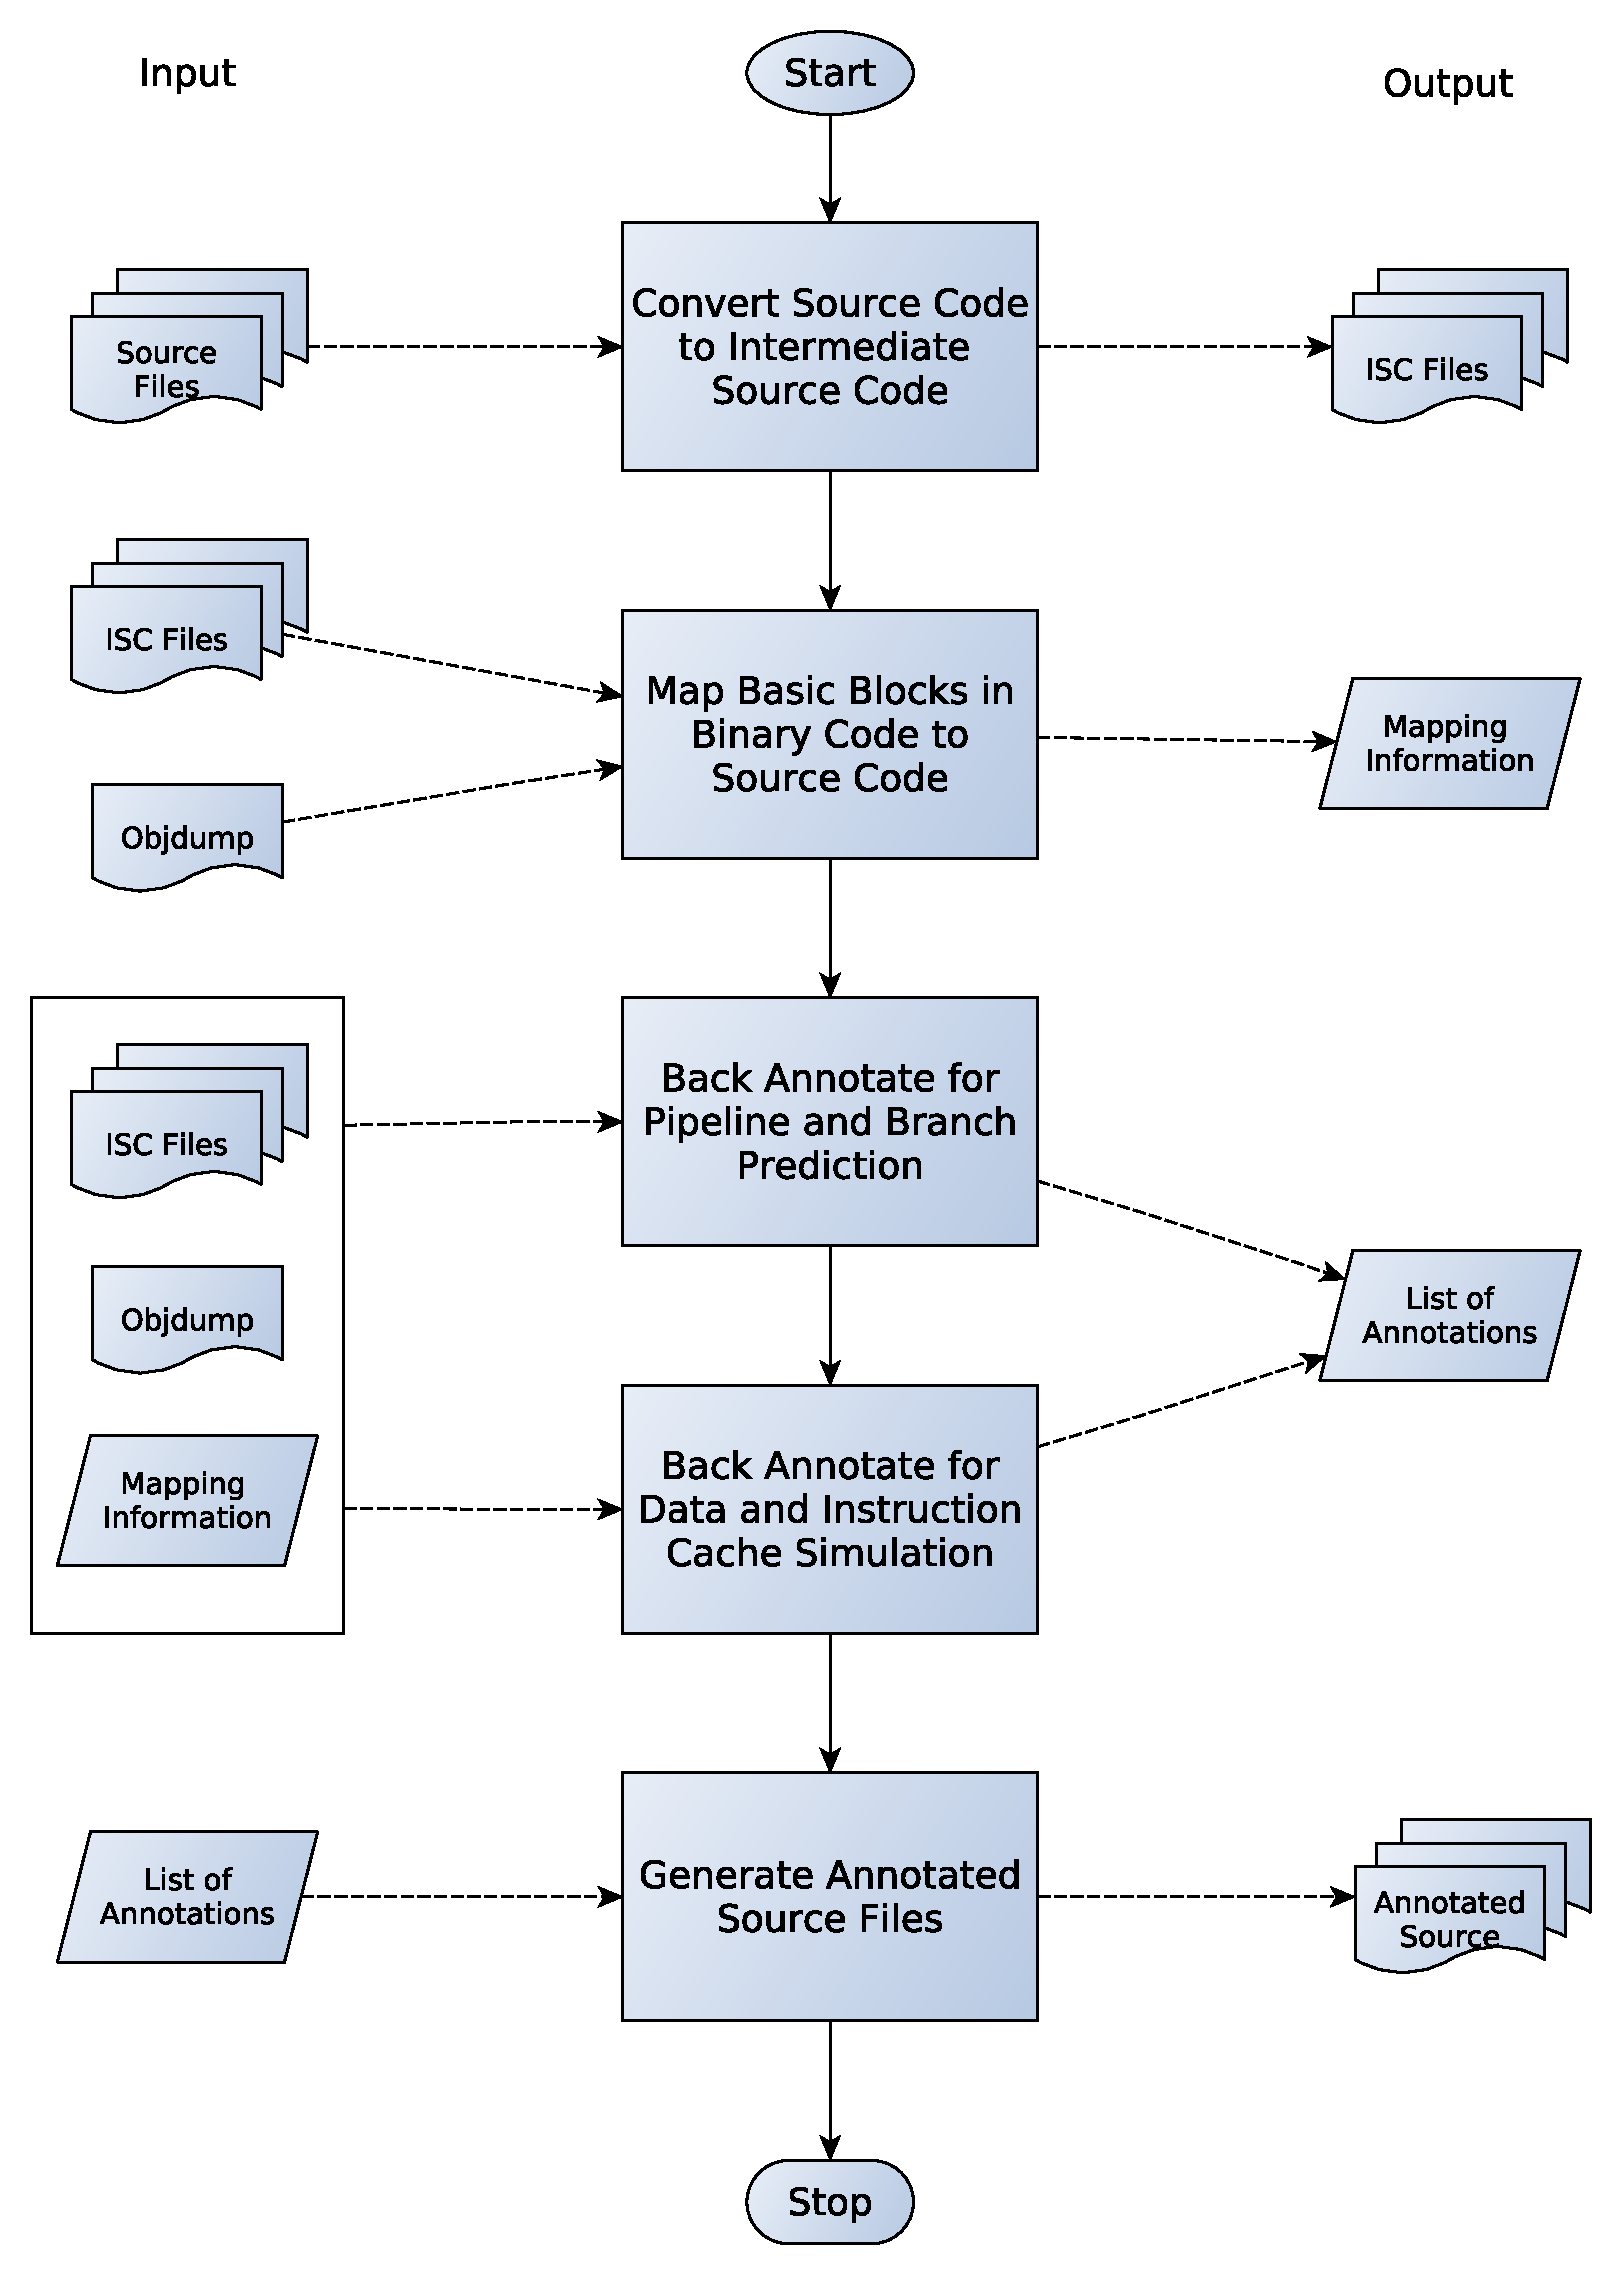
\includegraphics[width=.78\textwidth]{figures/HCS_FlowChart.pdf}
\caption{Flow Chart}
\label{fig:hcsFlowChart}
\end{figure}

In this section, a brief overview of the project architecture is provided. Each part of the project is independent, and has been treated as a separate problem. The flow chart in figure [TODO] shows each step of the project. The approach to solve these techniques is presented in the subsequent sections in this chapter. Details of the implementation have been presented in the next chapter.

From the example, it is clear that for correctly instrumenting the code accurate mapping is required between the source code and the binary code. However, this mapping is usually destroyed during the optimization phases of the compiler. The first problem that is solved in this project is to generate accurate mapping information at the Basic Block granularity. 

In the next step, GDB is used to derive information about each variable that is used in the application. During compiler optimization, most of the variables defined by the user are optimized out, hence this information can only be extracted from the debug information with the binary code. Names, addresses and sizes of Global and Local Variables are extracted.

For simulating data cache, each load and store instruction is accurately matched to an instruction in the source code. The variable being accessed is identified, and the annotation to simulate the memory access is added to the code. For simulating the instruction cache, annotation is added for each basic block in the binary code to the corresponding basic block in the source code.

To estimate the amount of cycles spent in execution of a basic block in the processor pipeline, each instruction in a basic block is sequentially parsed to identify interlocking. Interlocking occurs when there is a Control or Data Dependency between instructions, which results in pipeline stall for a few cycles. The cycles used by each basic block are annotated back to the code. Further, a mechanism to emulate Branch Prediction Unit has been implemented. 

\section{Source Code to Intermediate Source Code}
From the example, it is clear that mapping between source code and binary code is very important for accurate instrumentation. Unfortunately, this mapping is destroyed during the optimization phases of the compiler. The compiler optimizes code by moving instructions around, eliminating branch instructions and modifying loops. Some of these optimization strategies have been discussed in Section [TODO].

The compiler performs these optimizations in two stages. The front-end of the compiler, translates the source code from a high-level language like C, to an Intermediate Representation (IR) called GIMPLE. The processor independent optimization strategies are applied to the IR code. In the back-end of the compiler, the optimized IR code is translated into Machine Language for the target processor. The processor dependent optimization strategies are applied in this phase.

The Intermediate Code is expected to have a control flow similar to the control flow of the Binary Code, since most optimization strategies have already been applied. It should be much easier to perform mapping between the IR Code and the Binary Code. However, instrumentation of IR Code is difficult. 

In this project, the source code of the benchmark application is cross-compiled, and the optimized IR Code is translated back into a high-level language, C. The generated code is called Intermediate Source Code (ISC). The generated code is optimized version of the source code, with exactly similar functionality. It is easier to parse and instrument.

This approach is inspired from the research published in [TODO]. The python tool to translate GIMPLE code to C Code has been reused with minor modifications.

\section{Mapping Algorithm}
For accurate instrumentation, mapping at the Basic Block granularity is needed. GDB provides mapping information, but this has been observed to be highly inaccurate. This is a challenging problem and considerable research has been performed to develop algorithms for extracting accurate mapping.

The compilers employ a number of optimization strategies in which the control flow of the source code is modified. One such strategy is briefly discussed below, to illustrate the complexity of the mapping problem. Listing \ref{lst:cIfElse} shows a simple \emph{if-then-else} construct written in C. The code checks if \emph{a} is greater than \emph{b}. If true, the value of \emph{a} is assigned to \emph{max}, else the value of \emph{b} is assigned to \emph{max}.

Listing \ref{lst:objIfElse} is representative of how the assembly code may look like without any optimization.

\begin{center}
\begin{minipage}{0.7\textwidth}
\begin{lstlisting}[caption={Example C Code},label={lst:cIfElse}][h]
int max(int a, int b)
{
    int ret;
    if (a > b)
        max = a;
    else
        max = b;
    return ret;
}
\end{lstlisting}
\end{minipage}
\end{center}

\begin{center}
\begin{minipage}{0.7\textwidth}
\begin{lstlisting}[caption={Object Code},label={lst:objIfElse}]
00008068 <max>:
    8068:       cmp     r1, r0
    806c:       ble     8078   
    8070:       mov     r0, r1
    8074:       b       807c
    8078:       mov     r0, r0
    807c:       bx      lr
\end{lstlisting}
\end{minipage}
\end{center}

Each instruction is loaded in the processor pipeline. While the compare instruction on line 4 is being executed, the branch instruction on the next line is loaded into the pipeline. Depending on the result of the compare instruction, the branch will be taken or not taken. Since the result of the compare instruction is not yet available, the move instruction on line 6 is loaded into pipeline by assuming that the branch will not be taken. However, if the content of register \emph{r1} is lesser or equal to that of \emph{r2}, the pipeline will be flushed and move instruction on line 8 will be executed. The pipeline flush leads to a loss of a few cycles.

To reduce this loss, the Instruction Sets of most modern processors support a mechanism known as Predication or Conditional Execution. Each instruction like \emph{mov} or arithmetic instructions can be predicated with a condition. The instruction is loaded into the pipeline, but the result is only written back (or committed) if the condition evaluates to true. This feature can be used to eliminate conditional branch instructions. The optimized binary code is as shown in Listing \ref{lst:objOptimizedIfElse}.

\begin{center}
\begin{minipage}{0.7\textwidth}
\begin{lstlisting}[caption={Optimized Object Code},label={lst:objOptimizedIfElse}]
00008068 <max>:
    8068:       cmp     r1, r0
    806c:       movge   r0, r1
    8070:       movlt   r0, r0
    8074:       bx      lr
\end{lstlisting}
\end{minipage}
\end{center}

Since the branching instructions are eliminated, the code in Listing \ref{lst:objOptimizedIfElse} will be treated as a single basic block. The control flow graphs for the given source code, and the unoptimized binary code have been represented in figures \ref{fig:cfgSrc} and \ref{fig:cfgUnopt}. They are similar, and hence easy to map. Figure \ref{fig:cfgOpt} shows the Control Flow Graph of the optimized binary code. As expected, it is a single block. 

Similarly, other optimization strategies may modify the Control Flow. To map the Control Flow Graphs, a standard graph matching algorithm using Depth First Traversal has been implemented, and special handling has been done for each optimization strategy used by the compiler. Additionally, mapping information from GDB is used in corner cases.

\begin{figure}
\centering
\begin{subfigure}[t]{.33\textwidth}
\captionsetup{margin=10pt}
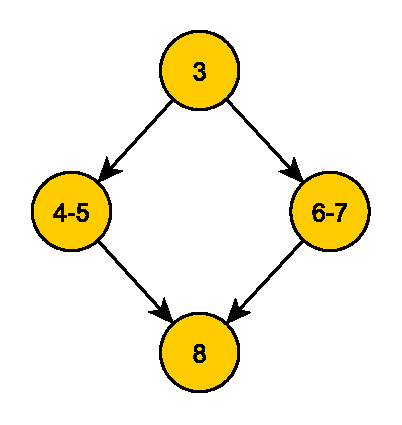
\includegraphics[width=\textwidth]{figures/CondExecSrcFlowChart.pdf}
\caption{Source Code}
\label{fig:cfgSrc}
\end{subfigure}%
~
\begin{subfigure}[t]{.33\textwidth}
\captionsetup{margin=10pt}
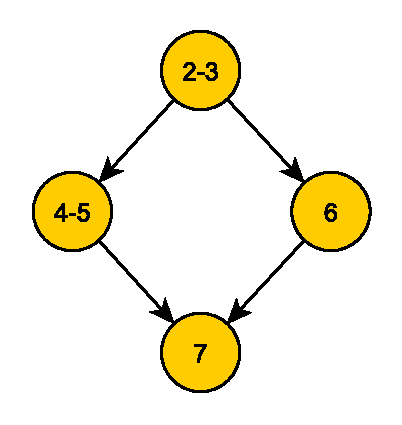
\includegraphics[width=\textwidth]{figures/CondExecObjUnoptFlowChart.pdf}
\caption{Unoptimized Binary Code}
\label{fig:cfgUnopt}
\end{subfigure}%
~
\begin{subfigure}[t]{.33\textwidth}
\centering
\captionsetup{margin=10pt}

\includegraphics[width=.5\textwidth]{figures/CondExecObjOptFlowChart.pdf}
\caption{Optimized Binary Code}
\label{fig:cfgOpt}
\end{subfigure}
\caption{Control Flow Graphs}
\end{figure}

During compile time, developers can tell the compiler which optimizations to perform using the option \emph{-O} followed by a number between 0 and 3 for the level of optimizations, 3 being the highest level of optimization. The tool currently provides promising results at optimization level 1, and can be extended to handle other optimization techniques.

The Control Flow Graphs generated from ISC and the Optimized Binary Code, along with the mapping information generated by the algorithm is stored in a data structure. The data is used in the next steps.

\section{Annotation for Execution Cycles and Branch Prediction}
The annotation for number of cycles spent in execution of the instructions is done at a basic block granularity. Cycles are estimated for each basic block in the binary code, and back annotated to the mapping block in the source code.

To accurately estimate the number of cycles spent in executing the instructions in a basic block, the pipeline architecture of the target processor must be understood. The target processor used for this research is ARM Cortex A5 which has an 8 stage pipeline. As is common with pipelined architectures consecutive instructions may face interlocking, which will lead to pipeline stalls.

Details about the architecture of ARM Cortex A5 are covered in Section [TODO].


\section{Extracting Debug Information from GDB}
\label{sec:C3GDBInfo}
As discussed briefly in the example, each load/store instruction in the binary code must be matched to a variable in the source code to simulate Data Cache Access. To be able to do this, information about each variable used in the code must be extracted. GDB has been used to extract this information.

Section \ref{sec:GDBInfo} describes how GDB can be used to extract names, addresses and sizes of each Global and Local Variable. GDB also offers a mechanism to use scripts, which operate a series of commands and generate an output, which can be later parsed to gather the information required. This mechanism of GDB has been used.

The tool automatically generates GDB scripts and runs them, to extract information about the variables used in the program. For each variable the following information is collected.

\begin{itemize} \itemsep -6pt
\item \texttt{name} of the variable
\item \texttt{scope} of the variable. Empty for Global Variables, name of the containing function for local variables.
\item \texttt{address} of the variable. For Global Variables it is the physical address. For local variables, it is the address relative to the Stack Pointer.
\item \texttt{type} of the variable.
\item \texttt{size} of the variable.
\end{itemize}

\section{Data Cache Simulation}
To estimate total time spent in fetching data from the memory, the tool performs detailed Cache Simulation. Each load/store instruction in the binary code is matched with to an instruction in the source code. The address from which the data is being fetched is identified, and memory access for the address is simulated. 

Generally speaking, the host and target processors may use a different memory layout. For example, in some processors memory needs to be allocated in an aligned fashion for better performance, however this may not be the case for another processor. Also, the sizes for the basic data types may differ among different architectures. Size of an integer in one architecture may be 4 Bytes and in another may be 2 Bytes. For accurate cache simulation, the address at which the variable resides in the Host Machine, can not be used. Instead, each memory access as it would occur on the target processor must be simulated.

The challenge lies in extracting the address from which the data is being fetched. This address can not be easily extracted from the cross-compiled binary by static analysis. To extract this address, the tool implements a mechanism to reconstruct each memory access as it occurs on the target processor. The approach is based on the research published in [TODO].

An application uses memory to read and write input and output data. For simplicity, let us consider how an application written in C Programming language uses memory. The memory can be used by the application in 3 ways. 

\begin{itemize} \itemsep -6pt
\item \textbf{Global Memory.} Data stored in Global Memory is accessible by all functions in the program. The memory is stored in a fixed size Data Section. Size of each Global Variable must be known at compile time, so it is called statically allocated memory. In bare metal applications, the physical address of each global variable is known after compilation, and can be extracted from the binary.
\item \textbf{Local Memory.} Each function can define variables which can only be used inside the function. The content of local variables is stored in the stack frame of the function. The size of the variable must be known at compile time. The addresses used by the local variables at run-time can not be known by static analysis, however the address relative to the Stack Pointer can be extracted.
\item \textbf{Heap Memory.} Applications can also allocate memory at run-time. The content of this dynamically allocated memory is stored in a special section known as Heap. The heap can grow and contract at run-time. The address and sizes of this type of memory can not be known statically. 
\end{itemize}

The current implementation of the tool, only focuses on simulating access from the Local and Global Memory. Cache Simulation for Heap Memory is complicated, because the memory allocation algorithm used in the target processors have to be emulated to know the exact address where the memory will be allocated. This means, that the tool can only be used with Benchmark applications that do not use Dynamic Memory. This does not limit the importance of this tool since the goal is to simulate for performance analysis, and not functional verification. %TODO: unnecessary last sentence?

The following section explains how each load/store instruction in binary code is mapped to a variable in the source code. Further, the approach to reconstruct the memory access is explained. Implementation of the cache simulator is explained in brief.

\subsection{Memory Access Reconstruction}
The tool parses binary code and emulates each instruction. It maintains the state of registers and updates it, as per the instructions. Branch instructions are ignored. The load/store instructions use register addressing modes to access data. From the content of the register the address of memory being accessed can be known. The memory being accessed may be an array, and this can not be clearly identified at this point.

The addresses of the Global Variables are known. Also, the addresses of Local Variables relative to the Stack Pointer are known. Using this information, the address of the load/store instruction found by emulation can be mapped to one of the variables.

Variables accessed in each basic block of the binary code are recorded, and this information will be used to map the load/store instruction to a specific line in the source code. For each basic block in the binary code, the basic block in the source code is parsed to find the line that causes the memory access. This is needed because the for accessing an array, the index to be added to the base pointer can only be extracted from the source code. 

Once this information is known, the memory address for each access can be reconstructed.

\subsection{Annotation for Data Cache Simulation}
\subsubsection{Global Variables}
For each Global Variable, say "\textit{var}" of any data type, another global variable "\textit{var\_addr}" of type "\textit{unsigned long}" is declared in the instrumented code to store the address where "\textit{var}" will be held in the target memory. This address was extracted using the method described in Section \ref{sec:C3GDBInfo}.

The line in the source code where the global variable is being accessed is identified using the technique presented in Section [TODO]. Instrumentation to simulate cache is added after this line. The Cache Simulator is implemented in C language. It offers the following API to simulate Data Cache Access.

\begin{lstlisting} [frame=none,numbers=none]
/**
 * @brief API Function to simulate Data Cache Access
 * 
 * @param address The address being accessed.
 * @param isReadAccess Flag to indicate type of access.
 * 					     True, if Read Access.
 * 					     False, if Write Access.
 *
 * @return number of cycles spent in performing the memory access.
 */ 
unsigned long long simDCache (unsigned long address, 
							     unsigned int isReadAccess)
\end{lstlisting}

The source code is appropriately instrumented using the above API. For accesses to elements in an array, the index multiplied by the size of the data type is added to the base address. The return value is the number of cycles spent in performing the memory fetch. This value is accumulated in a global variable, in a similar way as shown in the simple example above.

\begin{lstlisting}
int result;
unsigned long result_addr = 0x88ac;					// <--
int input_array[20];
unsigned long input_array_addr = 0x88b0;					// <--

void foo()
{
	
	
}
\end{lstlisting}

\subsubsection{Local Variables}
The approach for simulating access of Local Variables is quite similar to the approach used for global variables. A new local variable is declared for each local variable used in the function, with a suffix "\texttt{\_addr}" and data type "\texttt{unsigned long}". This variable contains the address of the local variable, relative to the current stack pointer. To accurately estimate the physical address where the memory resides, the value of the Stack Pointer is needed.

The stack grows and contracts during the run-time of an application. Whenever a function is called, a stack frame is created and the stack pointer is incremented. The stack frame contains the values of the function parameters, the local variables used in the function and the return address for the function. The size of the stack frame for each function can be extracted from the binary, and the start address of the stack is fixed at compile time. 

To maintain the value of the stack pointer, a global variable "\texttt{CSIM\_SP}" is added to the source code, which is initialized to the start address of the stack. At the beginning of each function, the value of "\texttt{CSIM\_SP}" is incremented by the size of the stack frame for the function. The address of the local variable, relative to the stack pointer is added to "\texttt{CSIM\_SP}", to calculate the physical address of the local variable, as would occur on the target processor.

The memory access is simulated using the same API as above.

\subsubsection{Function Parameters}
A func

\subsubsection{Register Spilling}

\subsection{Implementation of Cache Simulator}

\section{Instruction Cache Simulation}

\section{Annotation for Execution Time in Pipeline}

\section{Annotation for Branch Prediction}








